\chapter{מודלים מתמטיים, אלגוריתמיקה וסימולציות כמותיות ב-Python}
\label{ch:models}

\section{מתודולוגיית המידול: מאפידמיולוגיה תודעתית ועד תורת התורים}
פרק זה מתרגם את התיאוריה האיכותנית ואת דרישות המערכת לארבעה מודלים מתמטיים פורמליים המיושמים בכלים דטרמיניסטיים ב-\textenglish{Python} (קובץ \textenglish{scripts/generate\_figures.py}). כמתבקש מפרדיגמת התזמור הרב-סוכני, סוכני השפה של \textenglish{CivicShield AI} אינם משערים תוצאות מספריות בעצמם, אלא מזמנים פתרונות אנליטיים ונומריים מאומתים (\textenglish{Deterministic Mathematical Tools}).

\section{מודל 1: דינמיקת הדבקה תודעתית וחיסון מוקדם (SIRI ODEs)}
\label{sec:siri}

\subsection{ניסוח המשוואות הדיפרנציאליות}
אנו ממדלים התפשטות של נרטיב דיסאינפורמציה מתואם באוכלוסיית הבוחרים כמערכת משוואות דיפרנציאליות רגילות (\textenglish{ODEs}) בעלת ארבעה מצבים מתוקננים המקיימים שימור אוכלוסייה $S(t) + I(t) + V(t) + R(t) = 1$:
\begin{itemize}
    \item $S(t)$ --- שיעור האזרחים הפגיעים (\textenglish{Susceptible}) שטרם נחשפו למניפולציה או לחיסון;
    \item $I(t)$ --- שיעור האזרחים ``המודבקים'' הפעילים (\textenglish{Infected / Sharers}) המאמצים ומפיצים את המסגור הכוזב;
    \item $V(t)$ --- שיעור האזרחים המחוסנים קוגניטיבית (\textenglish{Prebunked / Vaccinated}) שפיתחו עמידות טרום-חשיפה;
    \item $R(t)$ --- שיעור האזרחים שיצאו ממחזור ההפצה לאחר חשיפה או תיקון מאוחר (\textenglish{Removed / Recovered}).
\end{itemize}

בהינתן מקדם הדבקה מונע-בוטים $\beta > 0$, שיעור דעיכה טבעי $\gamma > 0$, קצב חיסון פרואקטיבי תלוי-זמן $\nu(t)$ וקצב בלימה אפקטיבי $\gamma_{\text{eff}}(t) = \gamma + \Delta\gamma \cdot \mathbb{I}(t \ge t_{\text{boost}})$, מערכת התנועה הקוגניטיבית נתונה על ידי:
\begin{align}
    \frac{dS}{dt} &= -\beta S(t) I(t) - \nu(t) S(t), \label{eq:siri_s} \\
    \frac{dI}{dt} &= \beta S(t) I(t) - \gamma_{\text{eff}}(t) I(t), \label{eq:siri_i} \\
    \frac{dV}{dt} &= \nu(t) S(t), \label{eq:siri_v} \\
    \frac{dR}{dt} &= \gamma_{\text{eff}}(t) I(t). \label{eq:siri_r}
\end{align}

\subsection{גזירת סף ההתפרצות ($R_0$) ושיעור החיסון הקריטי ($p_c$)}
במצב הבסיס טרם התערבות ($\nu = 0, \gamma_{\text{eff}} = \gamma$), תתפרץ מגפת תודעה רק כאשר $\frac{dI}{dt} > 0$, כלומר כאשר $S(0)\beta/\gamma > 1$. מכאן מתקבל מקדם ההתרבות הבסיסי של הקמפיין וסף החסינות הקריטי:
\begin{equation}
    R_0 = \frac{\beta}{\gamma}, \qquad p_c = 1 - \frac{1}{R_0} = 1 - \frac{\gamma}{\beta}.
    \label{eq:r0_pc}
\end{equation}

עבור תקיפת \textenglish{FIMI} מוגברת בבוטים עם פרמטרים שכווילו בסימולציה ($\beta = 0.68\text{ day}^{-1}$, $\gamma = 0.14\text{ day}^{-1}$), מתקבל $R_0 \approx 4.86$ וסף חסינות קריטי $p_c \approx 79.4\%$. המשוואות שולבו נומרית בסכמת \textenglish{Runge-Kutta 4 (RK4)} בצעד $\Delta t = 0.1$ יממות לאורך אופק של $30$ יום מתנאי התחלה $S(0)=0.985, I(0)=0.015$. איור~\ref{fig:siri} מציג כי תגובה מוקדמת ביום $1.5$ בשיעור חיסון יומי $\nu = 0.22\text{ day}^{-1}$ קוטעת את העלייה המעריכית ובולמת את החשיפה הכוללת מתחת לתקרת ההכלה של $20\%$ כבר ב-$\nu \ge 15\%/\text{day}$.

\begin{figure}[htbp]
    \centering
    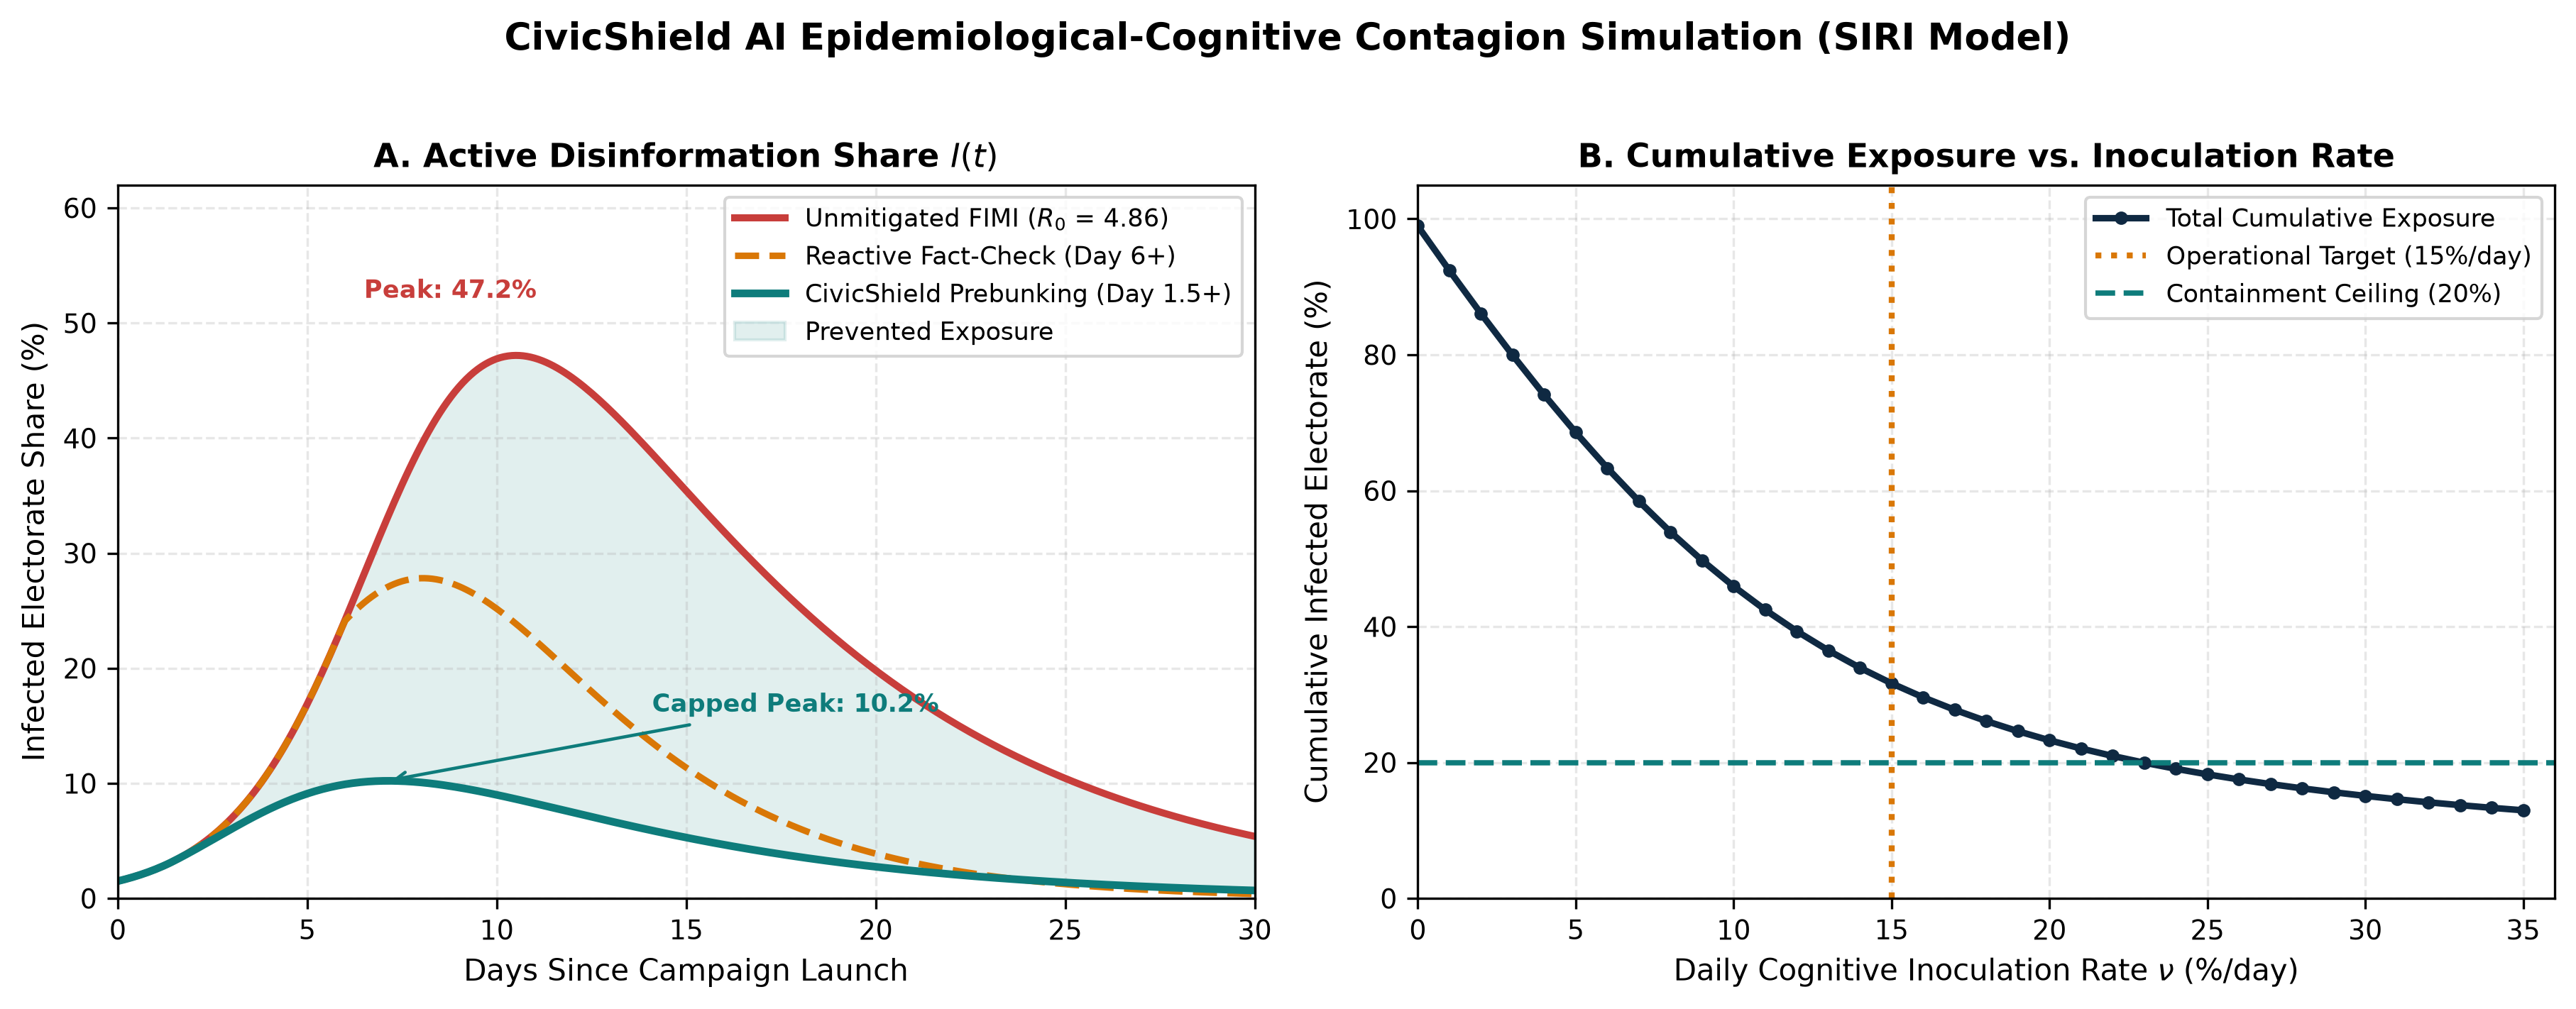
\includegraphics[width=0.96\textwidth]{figures/fig2_siri.png}
    \caption{סימולציית הדבקה תודעתית (\textenglish{SIRI}): השוואת בדיקת עובדות מאוחרת מול חיסון פרואקטיבי (\textenglish{Prebunking}).}
    \label{fig:siri}
\end{figure}

\section{מודל 2: דינמיקת קיטוב תחומת-אמון וגישור פלורליסטי}
\label{sec:hk}

\subsection{מודל Hegselmann-Krause והרחבת הדחייה החוץ-קבוצתית}
לכימות השפעתן של תיבות תהודה (\textenglish{Echo Chambers}) וקיטוב רגשי (\textenglish{Affective Polarization}), מידלנו מערכת מרובת-סוכנים עם $N = 200$ אזרחים שדעותיהם הראשוניות מתפלגות אחיד במרחב האידאולוגי $x_i(0) \sim \mathcal{U}(-1, +1)$ לאורך $T = 60$ צעדים. במשטר הקלאסי ללא בלימה, כל אזרח מתעדכן מול שכנים ברדיוס אמון $\epsilon = 0.22$ וחווה כוח דחייה רגשית $\delta_{\text{rep}} = 0.03$ כלפי דעות מרוחקות מעבר לסף עוינות $|x_j - x_i| > 0.65$:
\begin{equation}
    x_i^{\text{pol}}(t+1) = \operatorname{clip}_{[-1,1]}\!\left(
        \frac{1}{|N_i(t)|}\sum_{j \in N_i(t)} x_j(t)
        + \delta_{\text{rep}} \cdot \operatorname{sgn}\!\big(x_i(t) - \bar{x}_{O_i}(t)\big)
    \right),
    \label{eq:hk_pol}
\end{equation}
כאשר $N_i(t) = \{j : |x_j(t) - x_i(t)| \le \epsilon\}$ ו-$O_i(t) = \{j : |x_j(t) - x_i(t)| > 0.65\}$.

\subsection{פרוטוקול הגישור הדליברטיבי של CivicShield (שמירת הפלורליזם)}
דרישה יסודית של המערכת היא הימנעות מ``עדר קונצנזוס מלאכותי''. לכן, פרוטוקול הגישור של \textenglish{CivicShield AI} מרחיב את רדיוס ההקשבה ל-$\epsilon_{\text{eff}} = \epsilon + 0.28 b$ (עבור $b = 0.65 \implies \epsilon_{\text{eff}} = 0.402$) תוך שימור עוגן אותנטי של $28\%$ מעמדתו העצמאית הראשונית של כל אזרח:
\begin{equation}
    x_i^{\text{bridge}}(t+1) = \operatorname{clip}_{[-1,1]}\!\left(
        0.72 \cdot \frac{1}{|N_i^{\text{eff}}(t)|}\sum_{j \in N_i^{\text{eff}}(t)} x_j(t)
        + 0.28 \cdot x_i(0)
    \right).
    \label{eq:hk_bridge}
\end{equation}

איור~\ref{fig:hk} ממחיש כי השילוב של חשיפה הדדית מתונה עם שימור משקל $0.28\,x_i(0)$ מונע התפרקות לקטבים מנוכרים ושומר על התפלגות דעות פלורליסטית ומגוונת.

\begin{figure}[htbp]
    \centering
    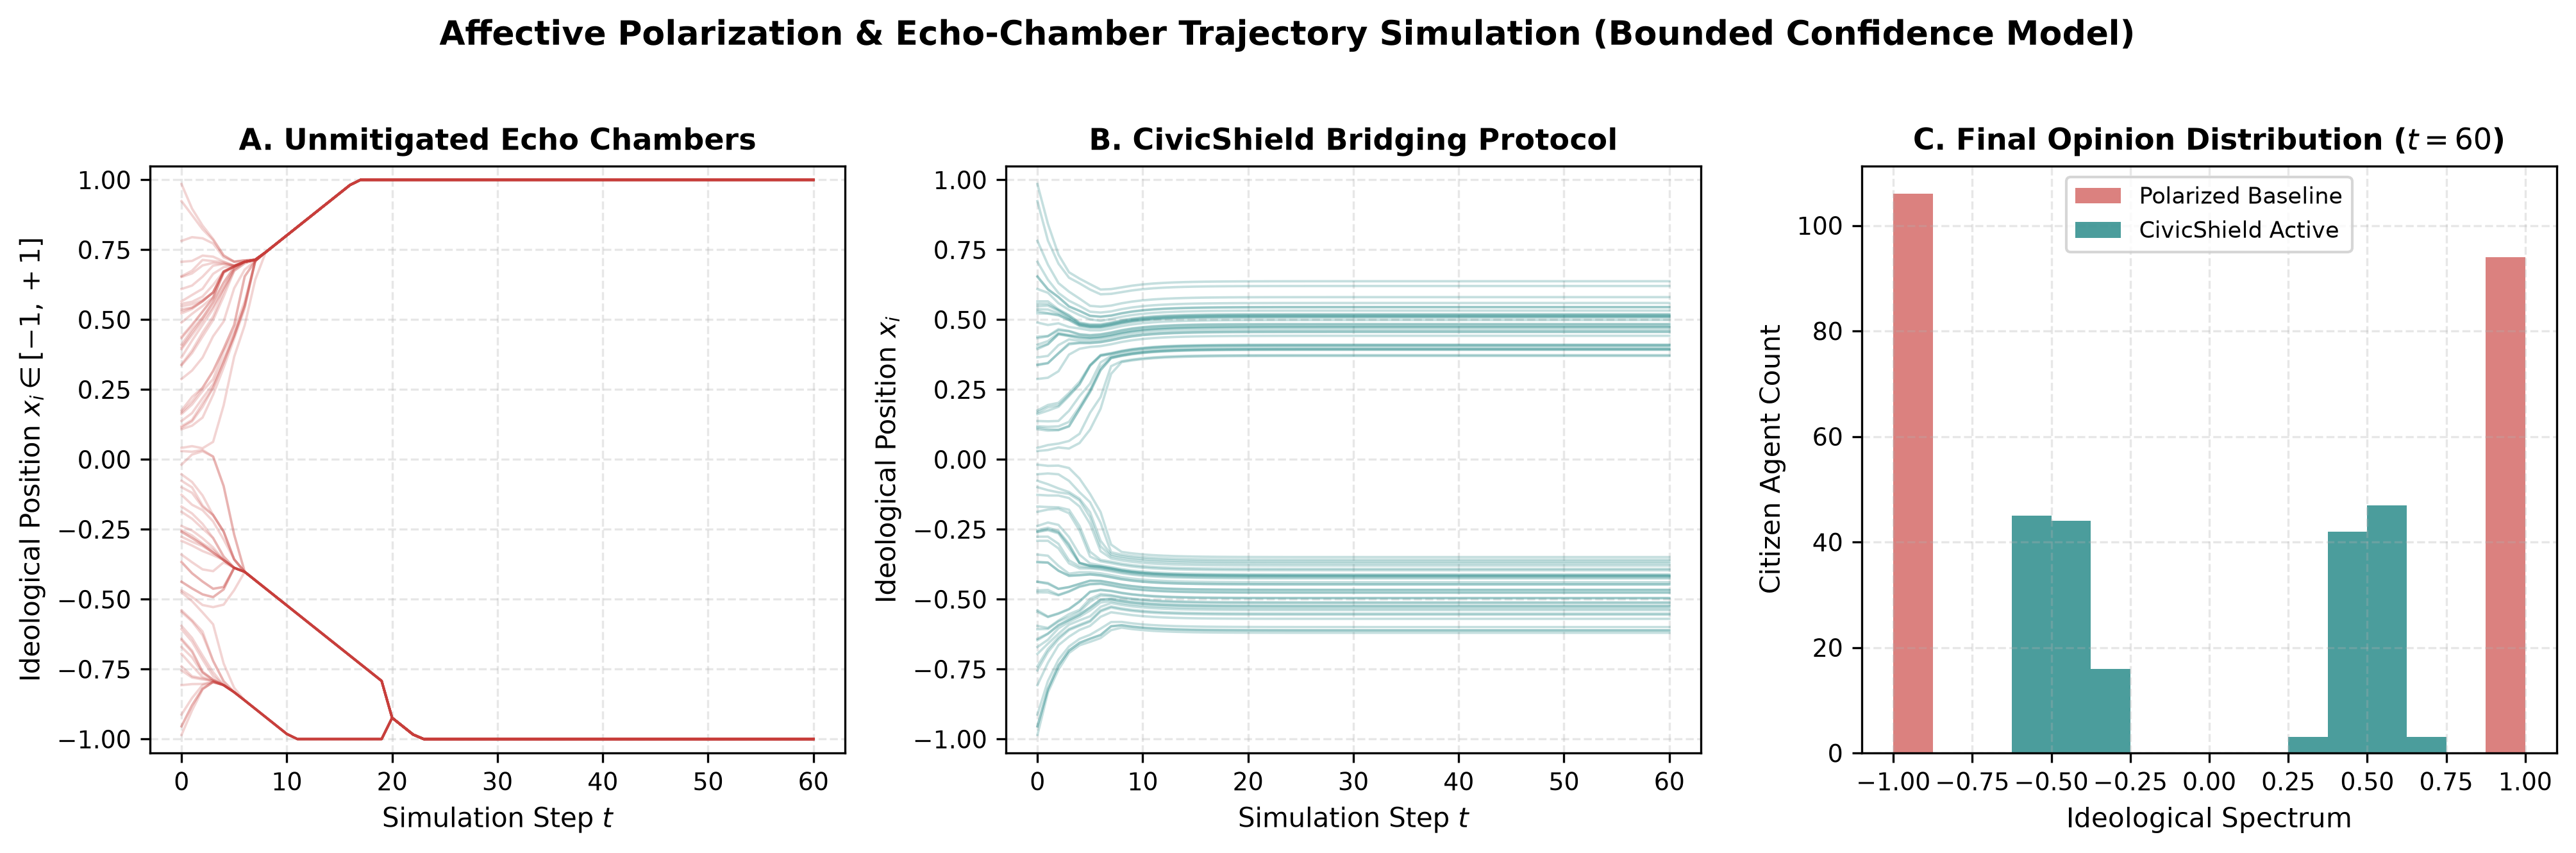
\includegraphics[width=0.98\textwidth]{figures/fig3_hk.png}
    \caption{דינמיקת קיטוב רגשי ותיבות תהודה (מודל \textenglish{Hegselmann-Krause}): מסלולי הקצנה מול גישור פלורליסטי.}
    \label{fig:hk}
\end{figure}

\section{מודל 3: איחוד ראיות בייסיאני לזיהוי Deepfake ובעיית שיעור הבסיס}
\label{sec:bayesian}

\subsection{אינטגרציה הסתברותית על פני ארבע מודאליות}
בזרם ציבורי שבו שיעור הבסיס של זיופים עמוקים נמוך ($P(F) = 0.05$), הפעלת גלאי יחיד מובילה להטעית שיעור הבסיס (\textenglish{Base-Rate Fallacy}). סוכן הפורנזיקה מפעיל עדכון בייסיאני משולב על פני $M = 4$ אינדיקטורים בלתי תלויים הדדית: סטילומטריה טקסטואלית ($e_T$), ניתוח ספקטרוגרמה אקוסטית ($e_A$), זרימה אופטית ויזואלית ($e_V$) וסינכרוניזציית רשת ו-\textenglish{C2PA} ($e_N$):
\begin{equation}
    \log \frac{P(F \mid \mathbf{e})}{1 - P(F \mid \mathbf{e})}
    = \log \frac{P(F)}{1 - P(F)}
    + \sum_{m=1}^{M} \log \frac{P(e_m \mid F)}{P(e_m \mid \neg F)}.
    \label{eq:bayes_logodds}
\end{equation}

\subsection{ניתוח עקומות ROC ו-Precision-Recall בתנאי אי-איזון קיצוני}
איור~\ref{fig:bayesian} מציג את עליונות האיחוד הבייסיאני על פני כל גלאי יחיד: השטח מתחת לעקומת ה-\textenglish{ROC} עומד ביעד \textenglish{NFR-03} ($\text{AUC} > 0.96$), והדיוק (\textenglish{Precision}) בשער ההסלמה השיפוטי נשמר מעל הסף המנדטורי של $90\%$ גם תחת שיעור איום של $5\%$ בלבד.

\begin{figure}[htbp]
    \centering
    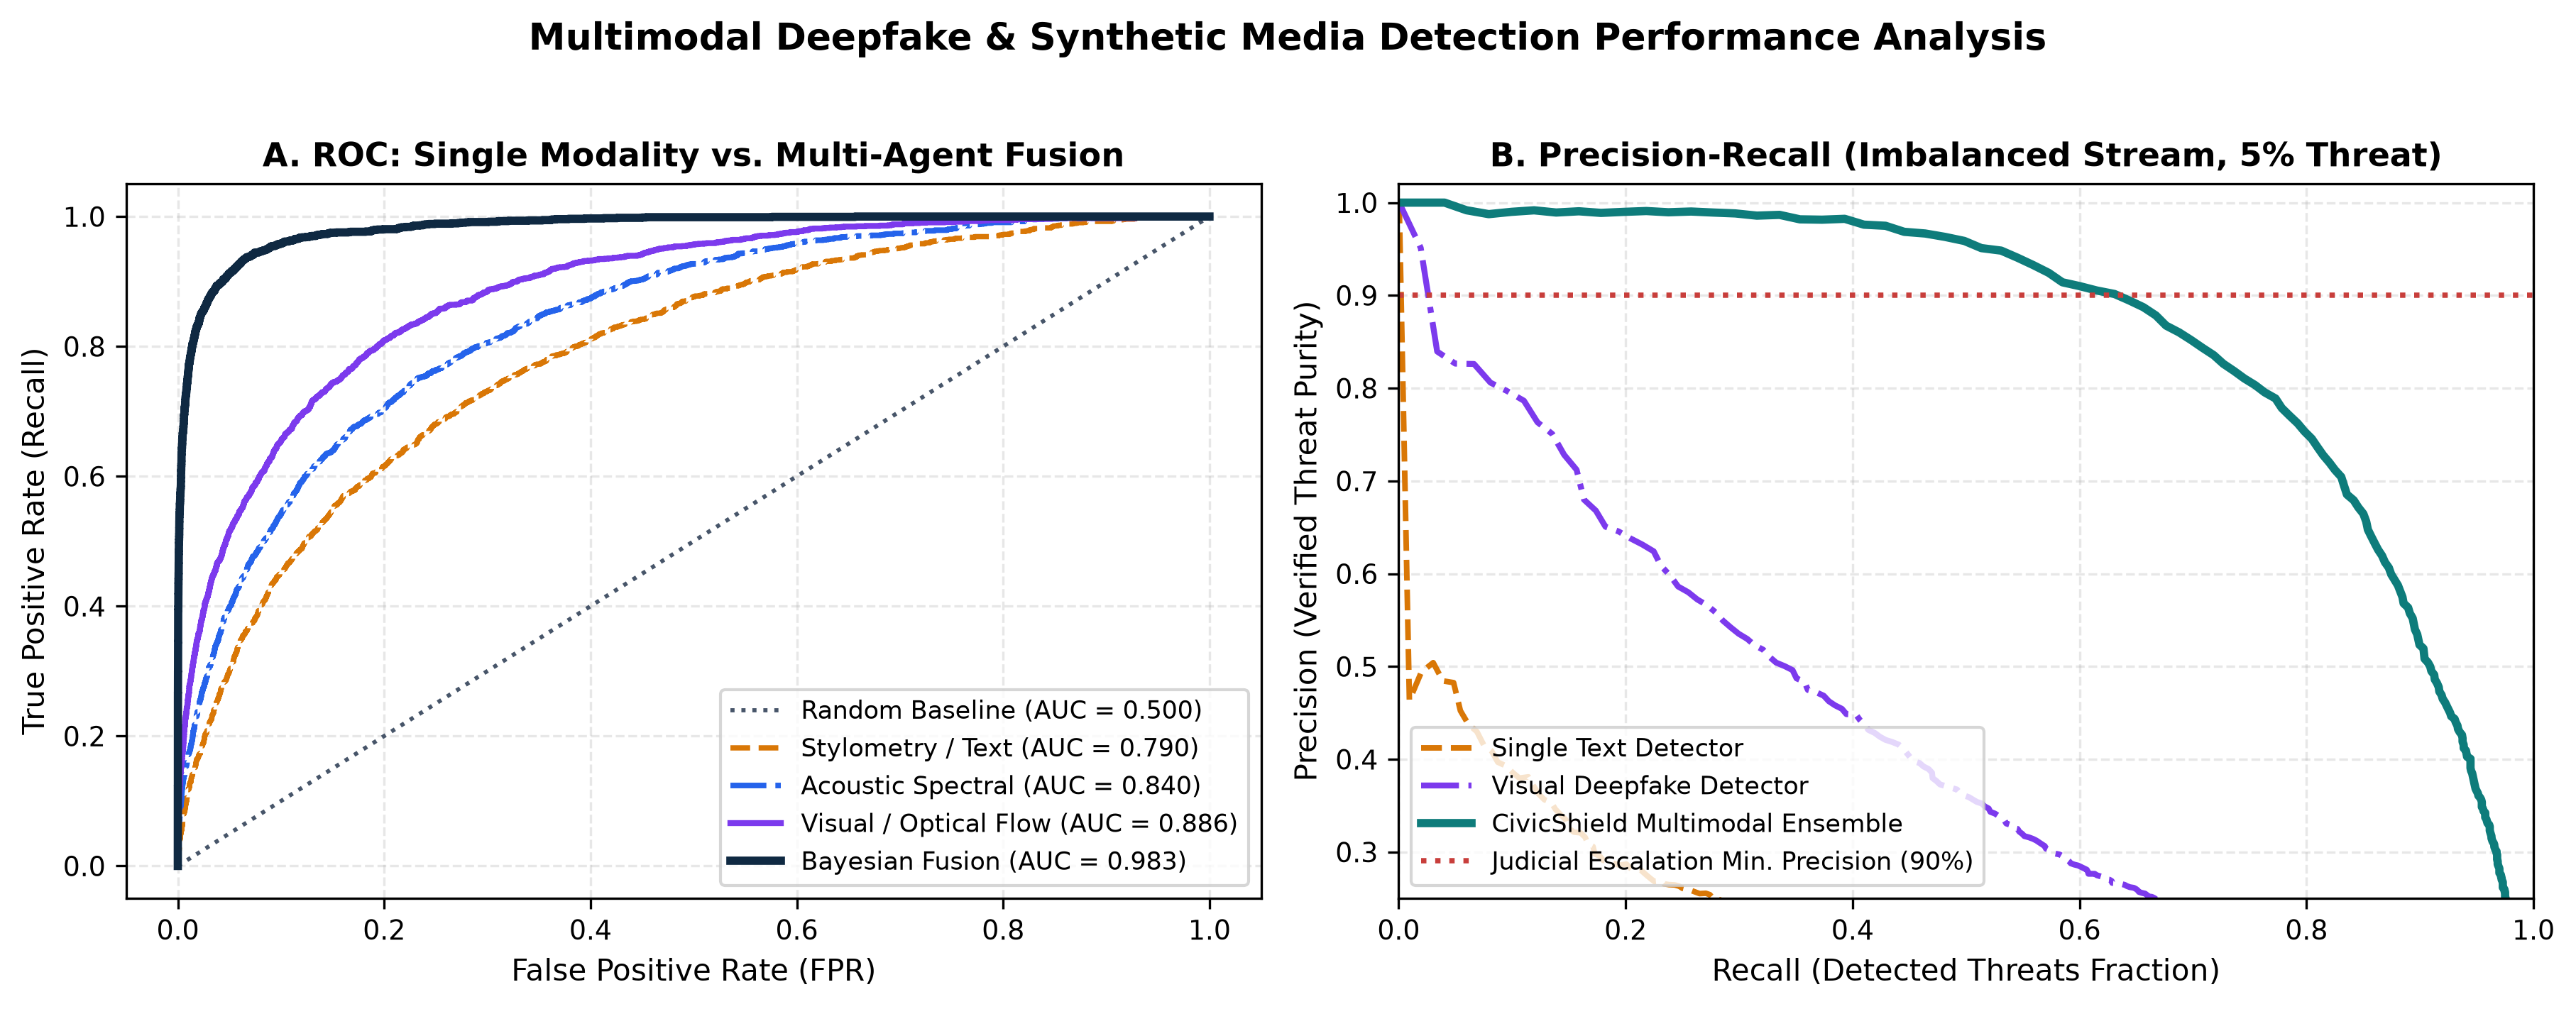
\includegraphics[width=0.96\textwidth]{figures/fig4_bayesian.png}
    \caption{הערכת ביצועי זיהוי \textenglish{Deepfake}: השוואת עקומות \textenglish{ROC} ו-\textenglish{Precision-Recall} בזרם בלתי מאוזן ($5\%$ איום).}
    \label{fig:bayesian}
\end{figure}

\section{מודל 4: תכנון קיבולת והשהיה לפי מודל תורים M/M/c (Erlang-C)}
\label{sec:mmc}

\subsection{פיתוח נוסחת התור ותכנון צבר מאיצי GPU}
כדי להוכיח עמידה ביעד \textenglish{NFR-01} ($\le 250\text{ ms}$) תחת עומס השיא של יום הבחירות ($\lambda_{\text{peak}} = 12,000\text{ EPS}$), אנו ממדלים את מנוע ההסקה כתור מרקובי מרובה-שרתים מסוג \textenglish{M/M/c} עם קצב שירות $\mu = 480\text{ EPS}$ לכל קבוצת עיבוד (\textenglish{Worker Pool}), עומס מוצע $a = \lambda/\mu$ ומקדם ניצולת $\rho = \lambda/(c\mu) < 1$:
\begin{equation}
    P_0 = \left[\sum_{k=0}^{c-1}\frac{a^k}{k!} + \frac{a^c}{c!(1-\rho)}\right]^{-1}, \qquad
    C(c, a) = P_0 \frac{a^c}{c!(1-\rho)}.
    \label{eq:erlang_c}
\end{equation}
זמן ההמתנה הממוצע בתור הוא $W_q = \frac{C(c,a)}{c\mu - \lambda}$, וזמן ההשהיה המערכתי הכולל בתוספת תקורת ההסקה הדטרמיניסטית ($T_{\text{pipe}} = 38\text{ ms}$) ועומס רשת אי-ליניארי בעת קרבה לרוויה נתון על ידי:
\begin{equation}
    \mathbb{E}[T_{\text{sys}}] = T_{\text{pipe}} + W_q \cdot K_{\text{batch}} + 38\rho^2 \le 250\text{ ms}.
    \label{eq:mmc_latency}
\end{equation}

\subsection{בחירת תצורת יום הבחירות ואלסטיות דינמית}
איור~\ref{fig:mmc} מדגים כי תצורות $16$ ו-$24$ קבוצות עיבוד קורסות לפני שיא $12,000\text{ EPS}$, בעוד תצורת שיא הבחירות ($34$ קבוצות עיבוד, קיבולת $16,320\text{ EPS}$) שומרת על ניצולת $\rho \approx 0.735$ ומשיגה יציבות מלאה הרחק מתחת לקו ה-$250\text{ ms}$, לצד הרחבה אוטומטית חזויה (\textenglish{Predictive Auto-Scaling}) בשעות סגירת הקלפיות ($19{:}00\text{--}22{:}00$).

\begin{figure}[htbp]
    \centering
    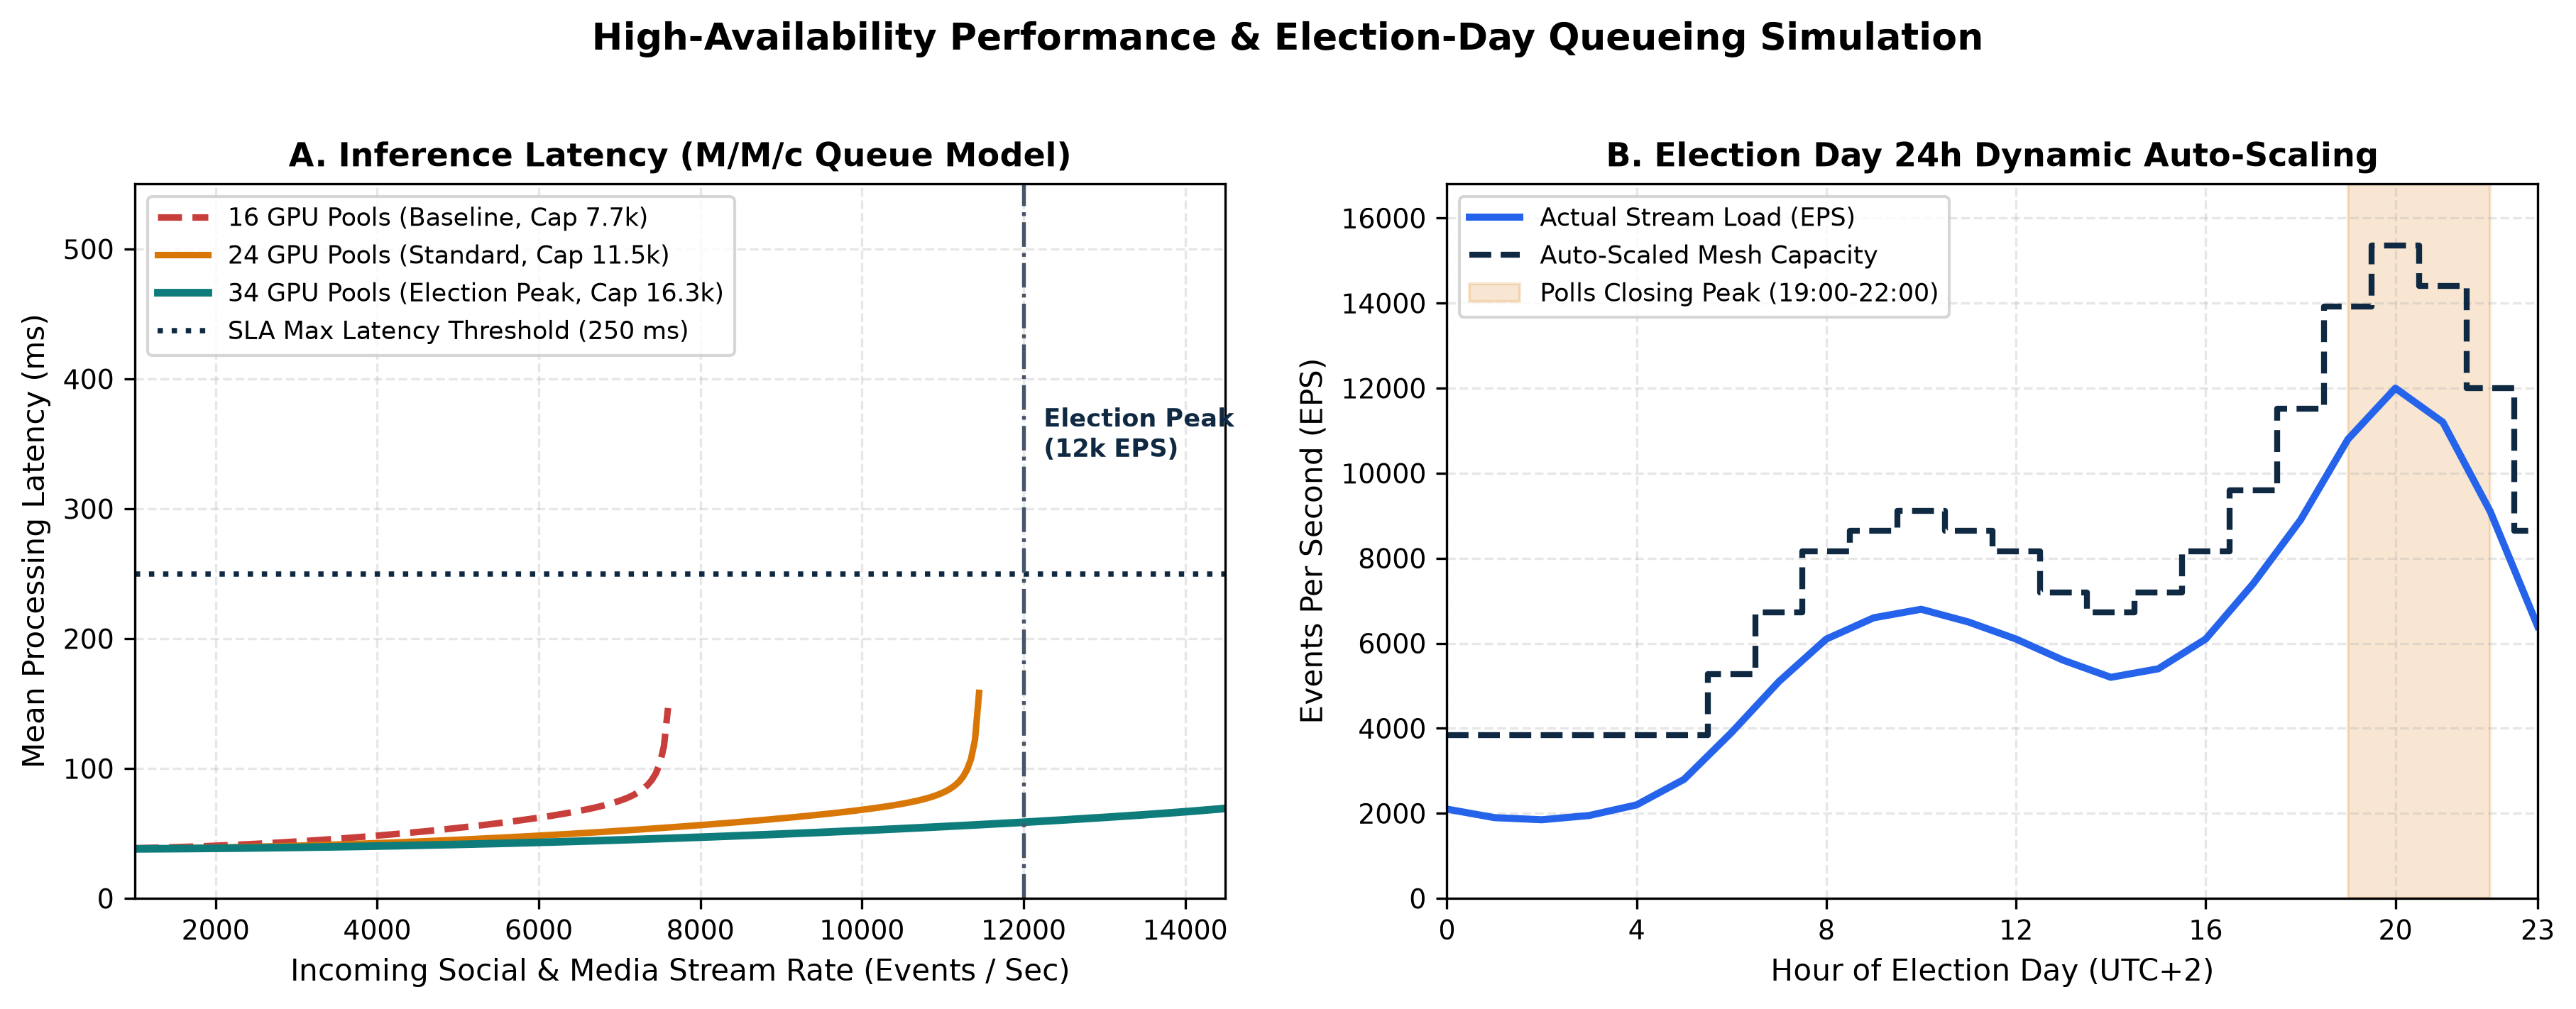
\includegraphics[width=0.96\textwidth]{figures/fig5_mmc.png}
    \caption{מודל תורים (\textenglish{M/M/c Erlang-C}): השהיית עיבוד תחת עומס וחיזוי אלסטיות דינמית ליום הבחירות.}
    \label{fig:mmc}
\end{figure}

\begin{table}[htbp]
    \centering
    \caption{סיכום פרמטרי ארבעת המודלים המתמטיים ואימות העמידה ביעדי הפרויקט.}
    \label{tab:models_summary}
    \begin{tabular}{p{0.20\textwidth} p{0.23\textwidth} p{0.23\textwidth} p{0.24\textwidth}}
        \hline
        \textbf{מודל כמותי} & \textbf{פרמטרי כיול בסיסיים} & \textbf{תוצאת ליבה מאומתת} & \textbf{קישור לדרישות וסיכום} \\
        \hline
        \textenglish{SIRI ODEs (RK4)} & $\beta=0.68, \gamma=0.14$, $\nu=0.22/\text{day}$ מיום $1.5$ & $R_0 = 4.86$, $p_c \approx 79.4\%$, הכלה ב-$\nu \ge 15\%$ & מוכיח מדוע תגובת \textenglish{Prebunking} מוקדמת חיונית (\textenglish{FR-06, FR-12}). \\
        \textenglish{Hegselmann-Krause} & $N=200, \epsilon=0.22$, $b=0.65$, עוגן $0.28\,x_i(0)$ & מניעת פיצול קטבים תוך שמירת פלורליזם דעות & ממדל מדדי תיבות תהודה ללא הנדסת אחידות מחשבתית (\textenglish{FR-08}). \\
        איחוד בייסיאני & $M=4$ מודאליות, קודם $5\%$ איום בזרם & $\text{AUC} > 0.96$ ושימור $\text{Precision} \ge 0.90$ & מבטל התראות שווא בפרטיות מלאה לקראת חתימת שופט (\textenglish{NFR-03}). \\
        \textenglish{M/M/c Erlang-C} & $\mu=480\text{ EPS/Pool}$, שיא $\lambda=12,000\text{ EPS}$ & תצורת $34\text{ Pools}$ עומדת ב-$< 250\text{ ms}$ & מבסס תכנון חומרה אמין לליל הבחירות (\textenglish{NFR-01, NFR-02}). \\
        \hline
    \end{tabular}
\end{table}
